\chapter{Introduction}

\section{Motivation}

From robots used for the automation of industrial processes to personal assistants robots and exploring robots for areas of difficult access, in the robotics area, we observe several applications with approaches from the least to the most complex in order to solve the most varied problems. Therefore, in order to develop the most distinct solutions, robotics appears as a multidisciplinary field, covering different lines of research, such as artificial intelligence, electronics, control, embedded systems, among many others.

One of the most prominent areas today is mobile robots, which aim to solve more complex tasks, in which the robot needs to move to carry out its activities. The difficulty of this branch is in how to control and coordinate the actions of robots so that they can interact with the environment and achieve their goal. For the accomplishment of some tasks, only one robot is not enough, being necessary then to use multiple robots, which makes the system more complex. Such systems prove how it is indispensable to have a control architecture for the coordination of all robots and a model of the organization of the system, capable of managing all the tasks that robots must perform, in order to achieve the system's objective, as can be seen in \cite{ACMultiplosRobos} and \cite{Moise}.

At the same time, in the line of development of control architectures for modeling intelligent agents in robotics, one of the fronts is the use of behavior trees to build the behavior of intelligent agents. Behavior trees were already widely used in the game development scenario, for modeling the behavior of non-playable characters, and, thanks to their modularity and flexibility, they have been gaining more and more notoriety in robotics \cite{BTsInRobotics}.

In this way, it is possible to take advantage of the structure provided by the behavior trees to model systems in which it is necessary to control the actions of several robots, being able to model both the behavior of the robots with behavior trees, as well as the organization that will coordinate all robots.

\section{Project Context}

\subsection{The ThundeRatz Robotics Team}

In order to develop national robotics and participate in academic competitions, the robotics team at Polytechnic School of the University of São Paulo was founded in 2001. This team, initially called \textit{Los Cuervos}, was reformed in 2005, giving rise to ThundeRatz \cite{ThundeRatz}.

Currently supervised by Prof. Dr. Rafael Traldi Moura, the group aims to learn about several topics that touch the state of the art of robotic systems, having contact with the newest lines of research. All this technical knowledge is used to design projects that encompass several areas of engineering, so that the team can put these projects to the test in national and international robotics competitions, gaining prominence on the robotics world stage.

At the moment, the team has several projects, having combat robots, sumo, hockey robots and autonomous robots that perform the most varied tasks, such as playing soccer or following a line on the ground.

\begin{figure}[!h]
    \centering
    
\includegraphics[width=.6\linewidth]{images/ThundeRatz Logo.png}
    \caption{ThundeRatz's logo. Taken from \cite{ThundeRatz}}
\end{figure}

\subsection{The IEEE Very Small Size Soccer (VSSS) category}

One of the most challenging and stimulating academic robotics competition categories is the \textit{IEEE Very Small Size Soccer (VSSS)} category. In it, competitors must develop an engineering solution for a team of robots that must play soccer autonomously, with each team composed of three players, each with maximum dimensions of 75 mm x 75 mm x 75 mm. The match is played on a 130mm x 150mm field and consists of two game periods, each lasting five minutes, with a half-time break of ten minutes.

Originally, the category had only its version with physical robots, in which matches are played on a black field with white markings and the robots have colored markings on their top, so they can be identified by means of a camera located above the field. However, due to the COVID-19 pandemic, the category adapted to the health context and also started to occur in a simulated environment, using the FIRASim \cite{FIRASim} simulator.

For the physical version, in addition to game strategies, the teams need to develop the mechanical and electronic system of the robots, as well as a computer vision system to identify the positions and speeds of the robots in the field and a communication system between the computer that runs game strategy and physical robots, for the transmission of movement commands.

As for the simulated version, there is no need to develop the systems relate to the physical world, only the system to determine the game strategy and a communication interface with the game simulator and with an automatic judge \cite{VSSReferee} developed for the category.

\begin{figure}[!h]
    \centering
    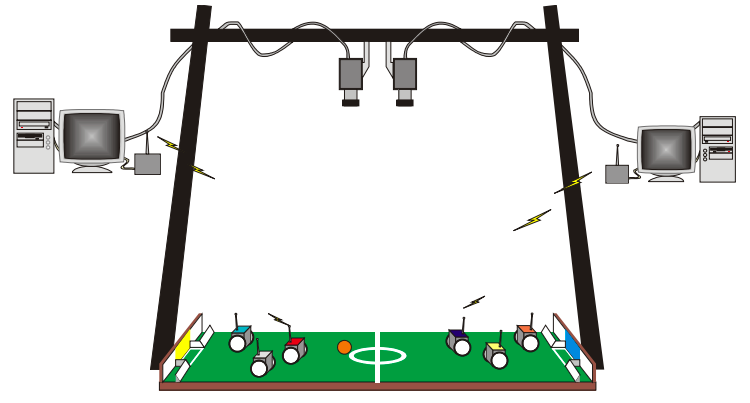
\includegraphics[width=.7\linewidth]{images/General System.png}
    \caption{Representative scheme of the system used in the category. Taken from \cite{FutRobosFerramentaDeEnsino}}
    \label{fig:general_system}
\end{figure}

\subsection{The ThunderVolt Team}

To participate in the \textit{VSSS} category, the ThundeRatz team developed a team of robots called ThunderVolt \cite{ThunderVolt} \cite{TDPThunderVolt}.

For its physical version, four robots were developed, called: Alan, Dorothy, Grace and Alex. Each inspired by a figure in science and engineering, with the honorees being, respectively, Alan Turing, Dorothy Vaughan, Grace Hopper and Alessandro Volta. In addition, a computer vision system was developed, using the library \textit{OpenCV} \cite{OpenCV}, and a communication system with physical robots, through the radio frequency modules nRF24L01 and an open source library developed by team \cite{STM3232RF24}. For its simulated version, a communication interface with the simulator and the automatic judge was developed using the UDP protocol.

\begin{figure}[!ht]
    \centering
    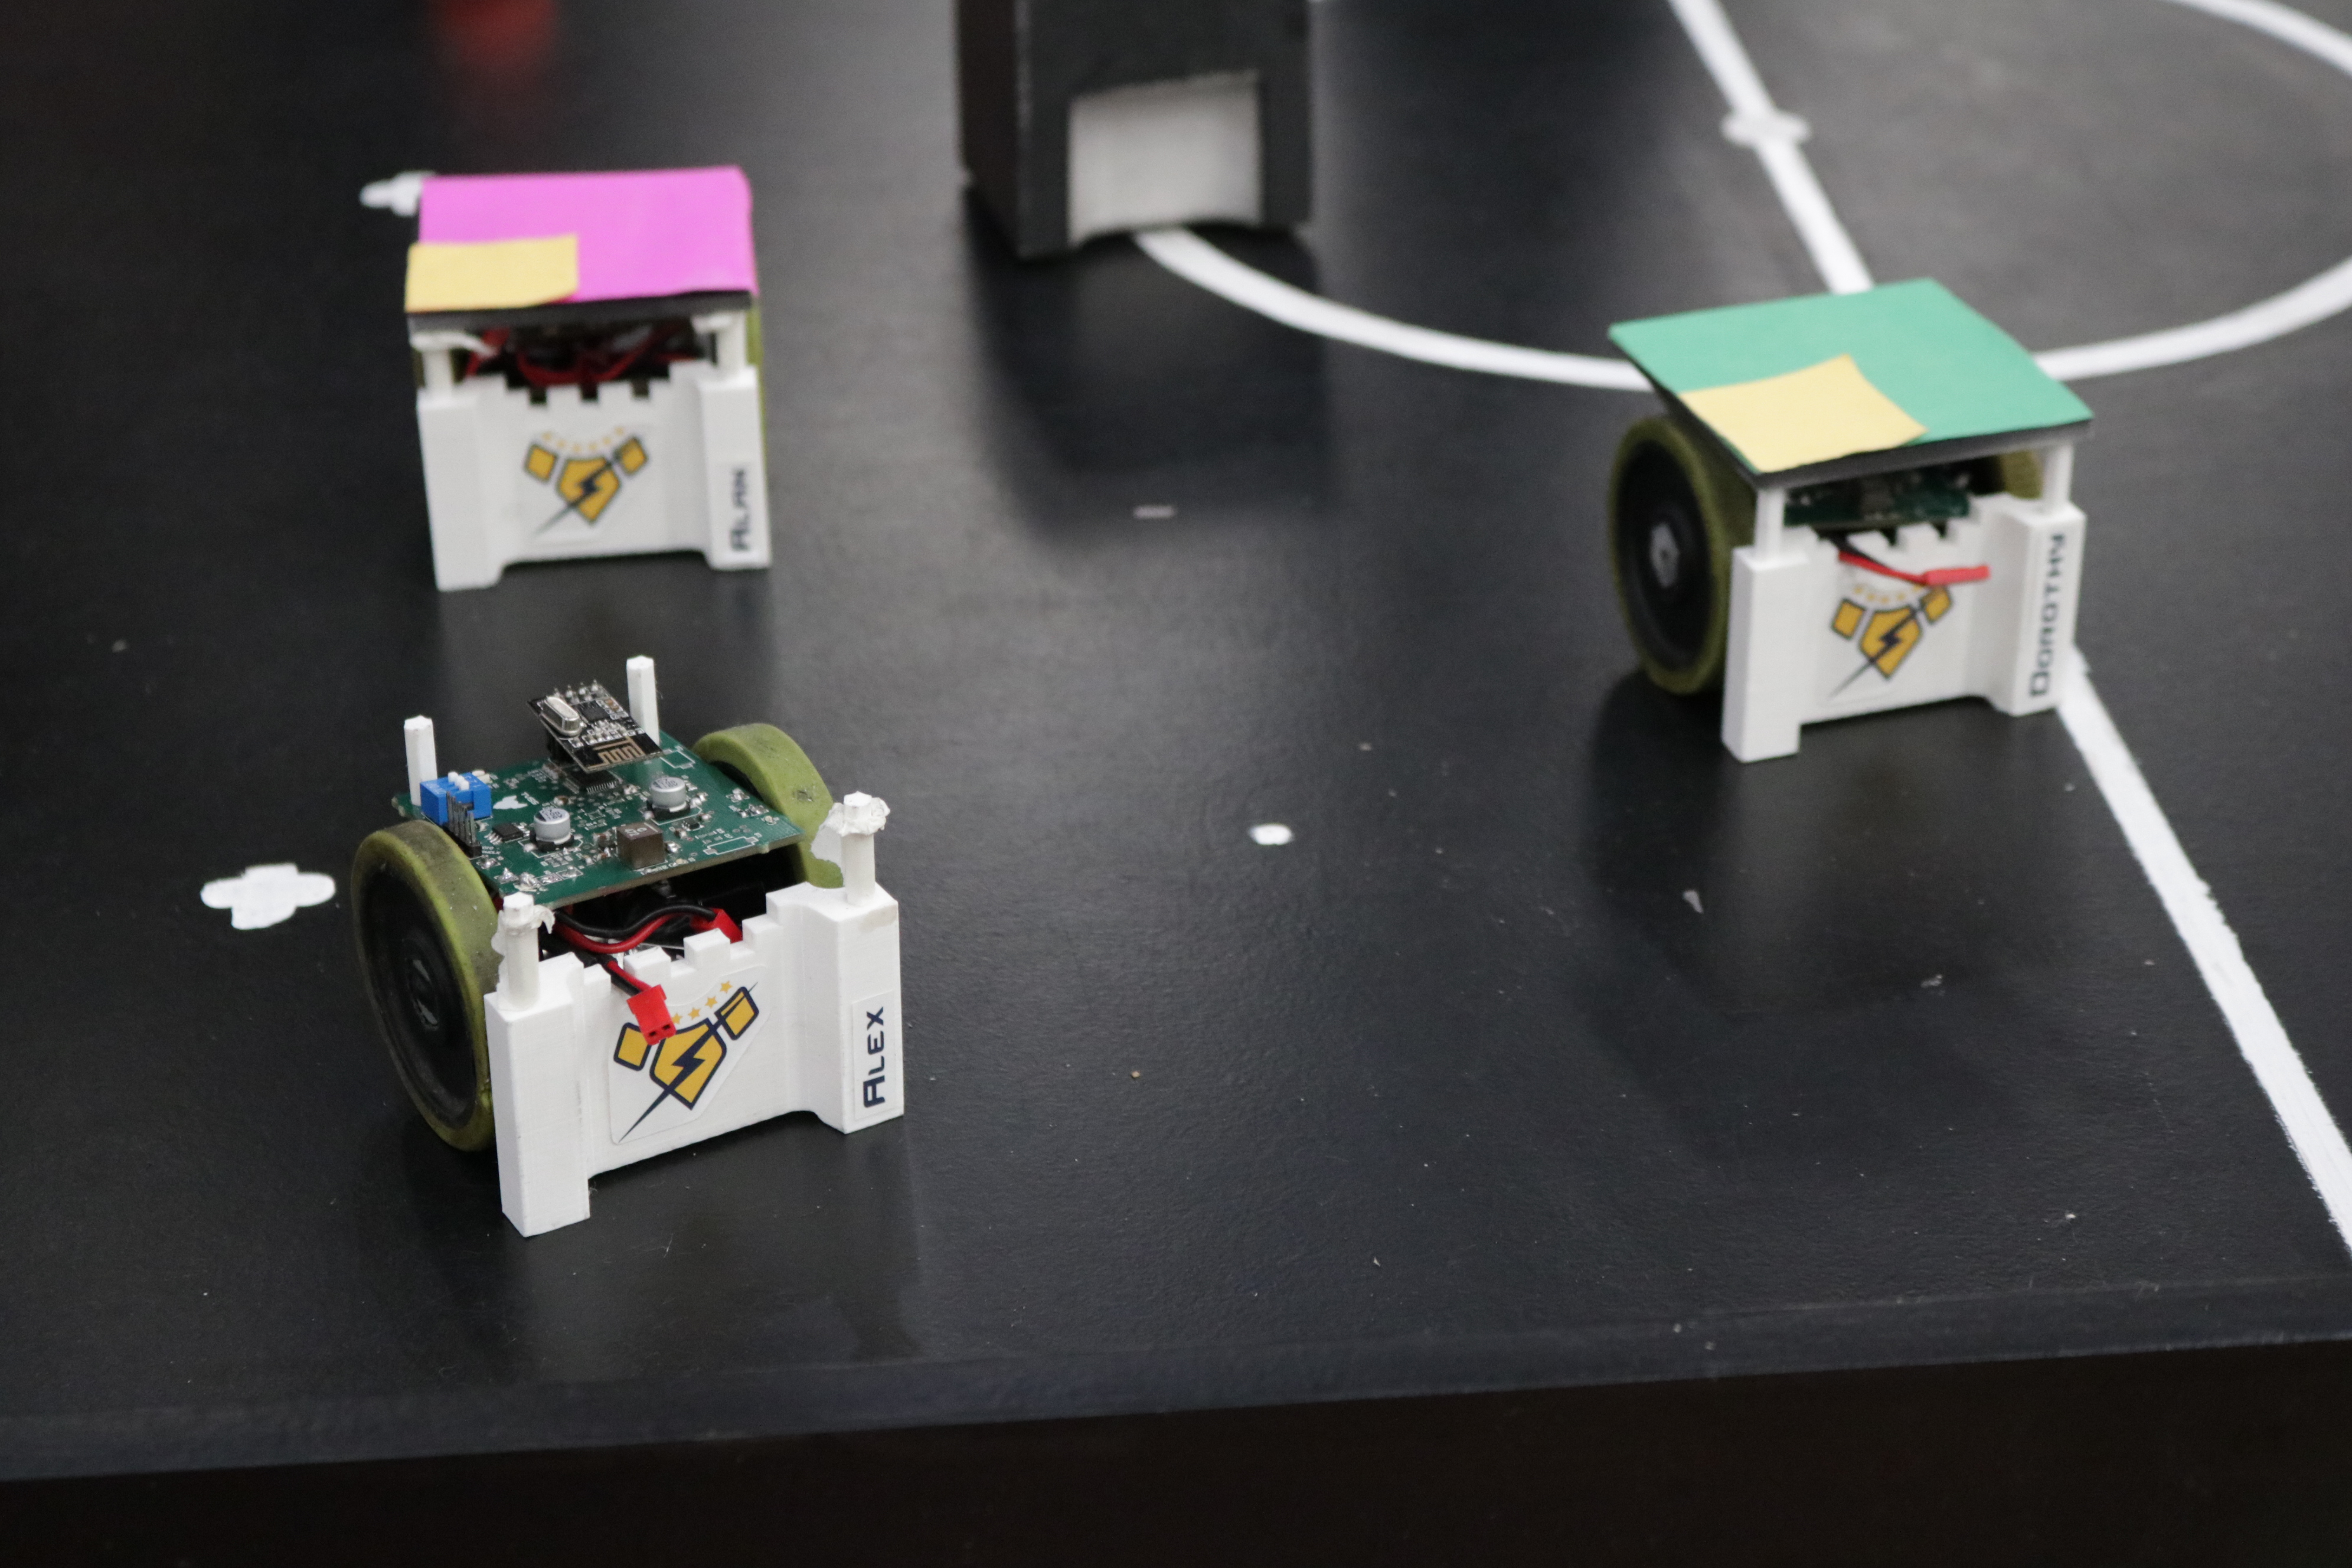
\includegraphics[width=.6\linewidth]{images/ThunderVolt Robots.jpeg}
    \caption{ThunderVolt team physical robots. Taken from \cite{ThunderVolt}}
    \label{fig:physical_robots}
\end{figure}

Regarding the central system that determines the strategy of the game and controls the behavior of the robots, it was implemented using the \textit{Robotic Operating System (ROS)} \cite{ROS}, a framework that provides several tools and libraries useful for developing robotics applications. Furthermore, to coordinate the team's actions, different technologies were used, such as methods of navigation through vector fields \cite{VectorFields} and behavior trees \cite{BTsInRobotics} to determine the behavior of each robot.

\section{Objectives}

This work aims to improve the architecture, maintainability and performance of the ThunderVolt team, in the competitions of the \textit{VSSS} category of autonomous robot soccer. Therefore, the intention is to introduce a new cooperation strategy based on an organizational model \cite{Moise} of agents, using behavior trees to model the structure of the organization and using the behavior of the existing agents. Thus, the objective of this work will involve the central system for determining the team's strategy, without impacting the other systems used in the project.

\section{Justification}

The use of the state of the art organizational model \cite{Moise} in combination with the use of behavior trees, which are a trend in the field of robotics \cite{BTsInRobotics}, guarantee a great opportunities for improvements in the ThunderVolt team, making the system more flexible, scalable and modular, thus enabling an improvement in its performance.

\section{Project Organization}

This work is currently divided into four chapters, with this introduction being the first.

In Chapter \ref{ch:methodology}, the project methodologies to be used in this work will be detailed, indicating the activities to be carried out and the goals.

In Chapter \ref{ch:target_system}, it will be described how the target system, the ThunderVolt team, works prior to the proposed changes, describing its current structure and the way it responds to external commands.

Finally, in Chapter \ref{ch:requirements}, the requirements of the team improvement proposal will be described.
